\section{Recovered supplementary exhibits from the source PDF}\label{app:recovered-exhibits}

This section preserves a compact set of supplementary exhibits from the source PDF while the author data and code remain unavailable. The assets are vector-preserving crops of the reported figures and tables, not regenerated results. Their purpose is auditability: a reader can compare the rewrite's characterization with the original display. Every exhibit must be replaced by a code-generated version before a claim of full replication or a final archival release.

\subsection{Inputs and predetermined characteristics}

\begin{figure}[p]
  \centering
  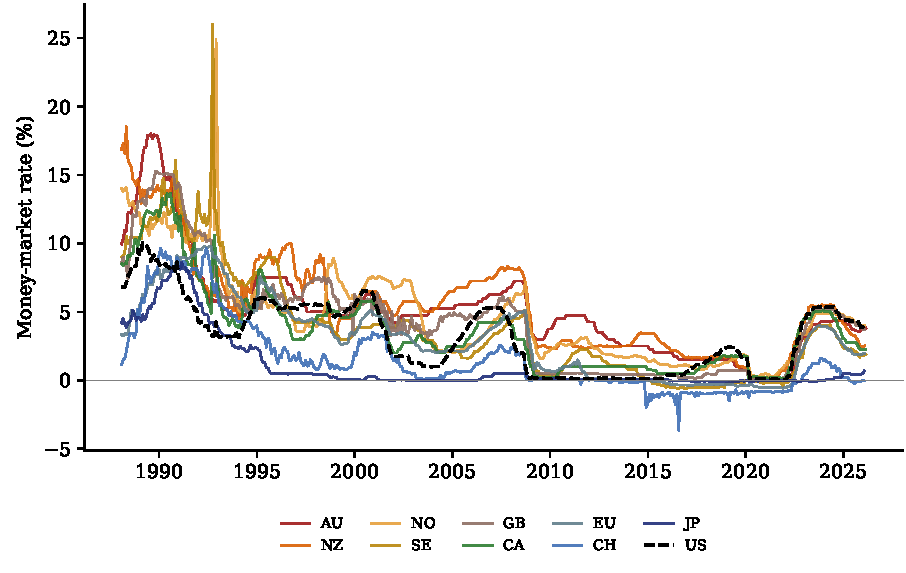
\includegraphics[width=\textwidth]{assets/original/figure_a01_appendix.pdf}
  \caption{Money-market rates in the inherited construction (source Figure A.1)}
  \label{fig:recovered-rates}
  \sourceNote{\inherited}
\end{figure}

\begin{figure}[p]
  \centering
  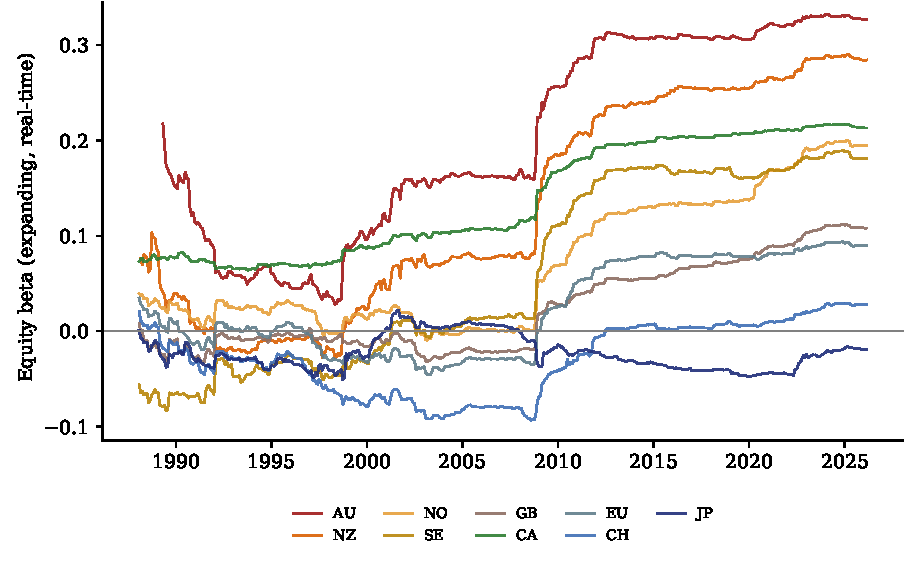
\includegraphics[width=\textwidth]{assets/original/figure_a02_appendix.pdf}
  \caption{Real-time expanding-window equity betas (source Figure A.2)}
  \label{fig:recovered-betas}
  \sourceNote{\inherited}
\end{figure}

\clearpage
\subsection{Specification neighborhood}

The next three recovered tables show the displayed cluster-size, exit-confirmation, and slope-definition variants. They document a local neighborhood, not the complete specification search. No multiplicity correction can be inferred from a displayed subset.

\begin{center}
  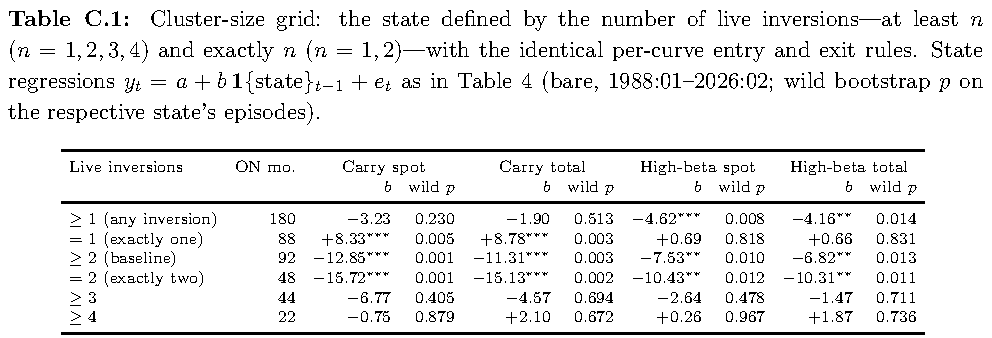
\includegraphics[width=0.98\textwidth]{assets/original/table_c01_appendix.pdf}
  \sourceNote{Source Table C.1. \inherited}
  \vspace{0.8em}

  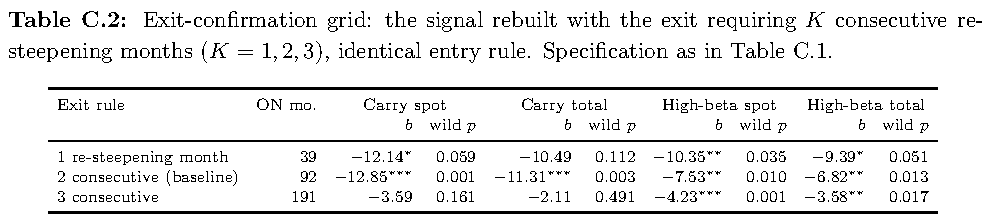
\includegraphics[width=0.98\textwidth]{assets/original/table_c02_appendix.pdf}
  \sourceNote{Source Table C.2. \inherited}
  \vspace{0.8em}

  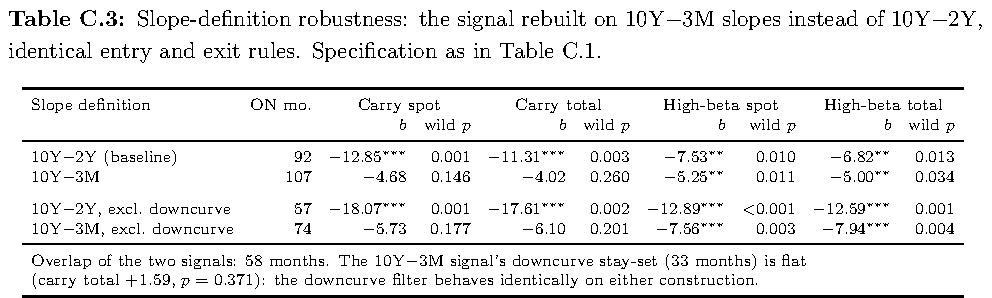
\includegraphics[width=0.98\textwidth]{assets/original/table_c03_appendix.pdf}
  \sourceNote{Source Table C.3. \inherited}
\end{center}

\clearpage
\subsection{Static counts, tail capture, and repairs}

\begin{figure}[!htbp]
  \centering
  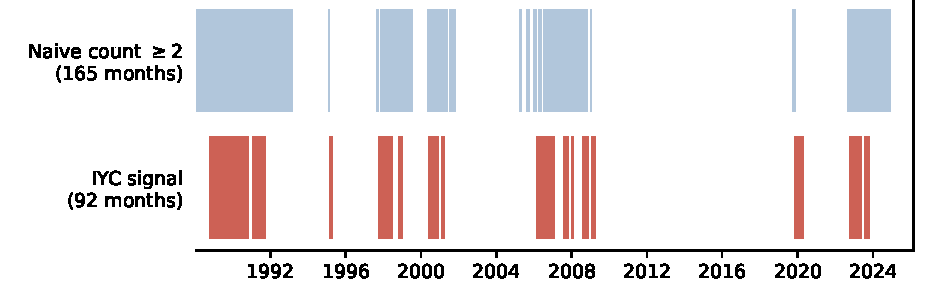
\includegraphics[width=\textwidth]{assets/original/figure_d01_appendix.pdf}
  \caption{Naive-count and latched-state timelines (source Figure D.1)}
  \label{fig:recovered-counts}
  \sourceNote{\inherited}
\end{figure}

\begin{center}
  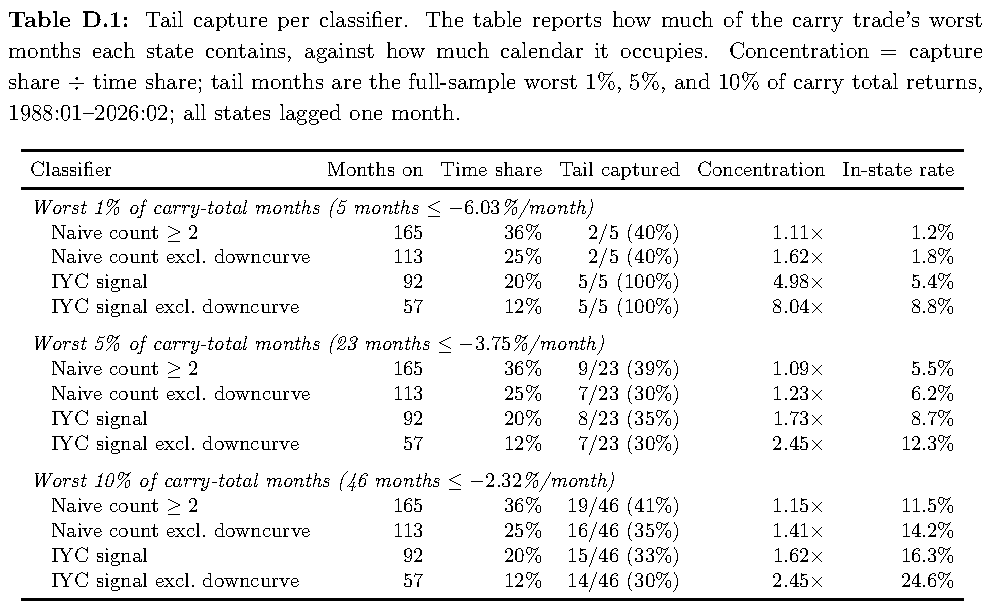
\includegraphics[width=0.98\textwidth]{assets/original/table_d01_appendix.pdf}
  \sourceNote{Tail capture at the 1, 5, and 10 percent thresholds, source Table D.1. \inherited}
\end{center}

\clearpage
\begin{center}
  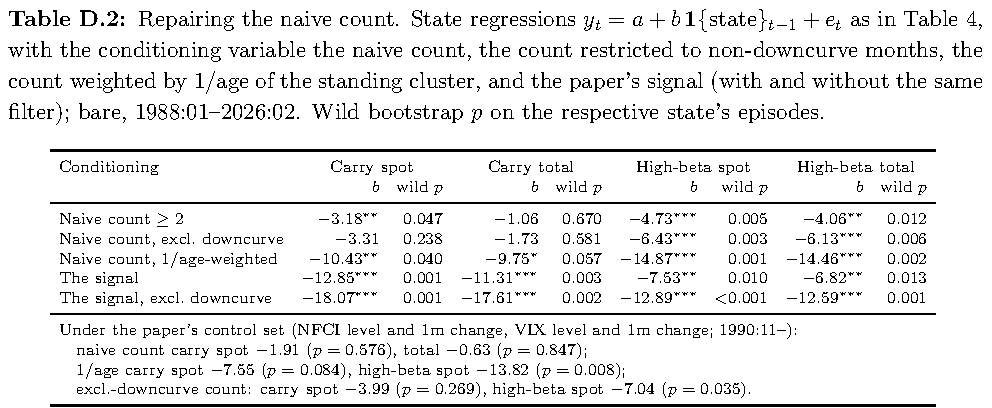
\includegraphics[width=0.98\textwidth]{assets/original/table_d02_appendix.pdf}
  \sourceNote{Naive-count repairs and controls, source Table D.2. \inherited}
\end{center}

\subsection{Calendar stability}

\begin{center}
  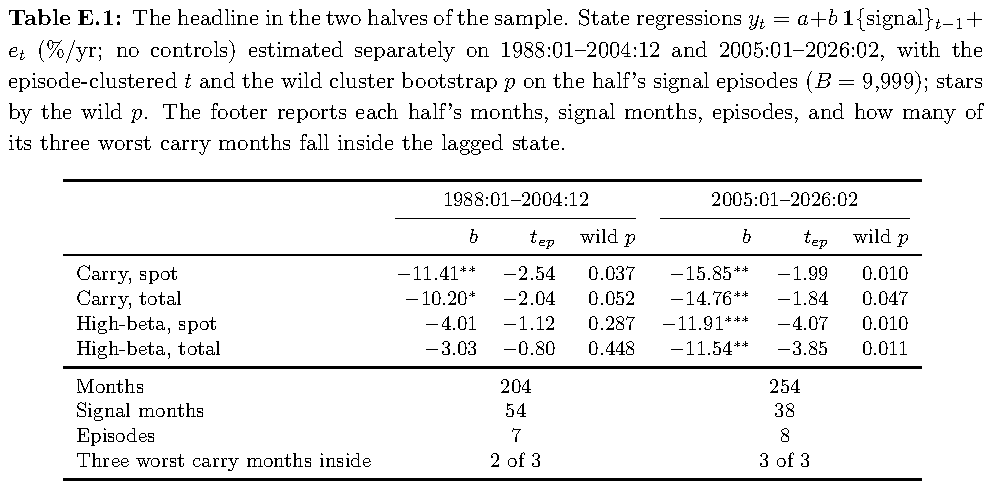
\includegraphics[width=0.98\textwidth]{assets/original/table_e01_appendix.pdf}
  \sourceNote{Two calendar halves, source Table E.1. \inherited\ The split is conditional on a full-sample-designed rule and is not historical out-of-sample validation.}
\end{center}

\clearpage
\subsection{Alternative local-projection designs}

\begin{figure}[!htbp]
  \centering
  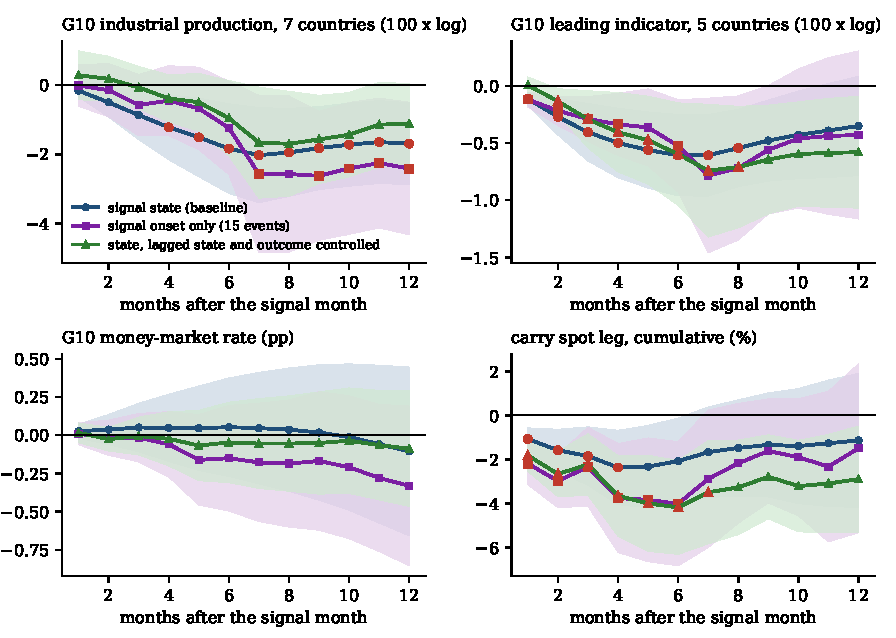
\includegraphics[width=\textwidth]{assets/original/figure_j01_appendix.pdf}
  \caption{Local projections under three inherited designs (source Figure J.1)}
  \label{fig:recovered-lp-variants}
  \sourceNote{\inherited\ Confidence bands and significance markers have not been regenerated.}
\end{figure}

\clearpage
\subsection{Common term-premium diagnostic}

\begin{center}
  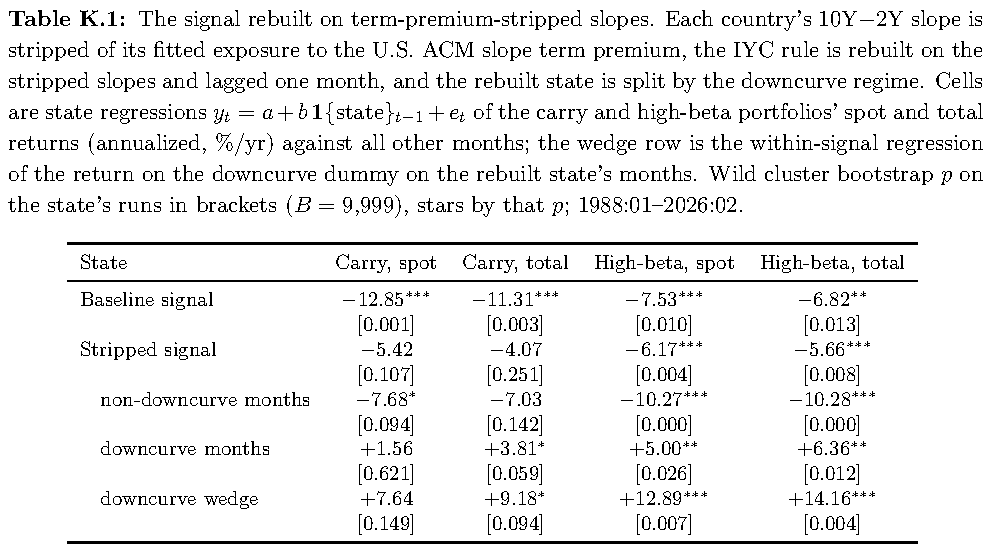
\includegraphics[width=0.98\textwidth]{assets/original/table_k01_appendix.pdf}
  \sourceNote{Term-premium-stripped signal, source Table K.1. \inherited\ The source uses a common U.S. ACM component; this does not remove country-specific foreign term premia.}
\end{center}

\clearpage
\subsection{Omitted source exhibits}

The source PDF also reports strategy overlays, emerging-market extensions, U.S.-inclusive variants, and portfolio-composition tables. They are catalogued in \path{rewrite/notes/figure_provenance.csv} and retained as audit assets under \path{rewrite/assets/original}. They are not reproduced here because they do not bear directly on the rewrite's single main contribution and because feasible forward returns, transaction costs, and the original portfolio code are unavailable. Omitting them from the narrative is a scope decision, not an adverse replication result.
